\documentclass[
  a4paper,
  % twocolumn,
  % draft
  ]{scrartcl}

% packages

  \usepackage{qbase}

  % extensions

    \bibliography{/Users/quirin/promo/bib/references}
    \usepackage{subcaption}

% new commands

  \newcommand{\lsil}[1]{\lstinline[language=Python]{#1}}
  \newcommand{\mtrc}[1]{\textcolor{blue}{#1}}

\begin{document}

% title

  \title{Social networks of lexical innovation}
  \subtitle{Investigating the diffusion of neologisms on Twitter}
  \author{Quirin Würschinger\\ LMU Munich}
  \maketitle

\listoftodos

\tableofcontents

% text body

\section{Introduction}

  \begin{easylist}[itemize]
    # \hw{Social media} has changed the way we communitate.
      ## It has changed the social fabric of our society (elections, press vs. \enquote{influencers}) and the sociolinguistic dynamics of how we communicate (fake news)
      ## It has also changed the language system and the way the language system changes. Much as \hw{cultural innovations} like XXX \enquote{go viral}, new digital modes of communication also affect the way \hw{linguistic innovations} spread. \todo{technical innovation, example like \ol{blockchain}}
      ## real viruses like Corona seem to spread similarly as linguistic innovations \enquote{go viral} \parencite{EandT2020}
    # This opens up new research questions and new ways to tackle previous questions in sociolinguistics. (sociolinguistics $\rightarrow$ computational sociolinguistics)
      # new data
      # new methods: social network analysis
    # research questions
      # How do new words spread?
      # Which factors influence their spread?
  \end{easylist}

\section{Theoretical background}

  \subsection{Modeling the conventionalization of lexical innovations}

    \begin{easylist}[itemize]
      # Research question: how do new words spread in the speech community?
      # previous perspectives
        ## \hw{structural}: language system, lexicalization, instutionalization, word-formation processes etc. \cite{Bauer1983,Lipka2005}
        ## \hw{cognitive} \parencite{Schmid2008}
        ## \hw{sociolinguistic}: S-curves \parencite{Labov2007,Milroy1992}
      # current framework: based on the EC-Model \parencite{Schmid2020}
        ## spread across usage contexts
        ## spread across speakers
    \end{easylist}

  \subsection{Investigation the conventionalization of lexical innovations empirically}

    \begin{easylist}[itemize]
      # Previous work has produced some important insights.
      # I focus on the sociolinguistic dimension of lexical innovation in this paper.
      # Previous empirical approaches have been limited in studying this because of the lack of information regarding the sociolinguistic dynamics of the spread of new words: how many speakers are affected? how are they interacting?
    \end{easylist}

    Overview of previous approaches

      \begin{easylist}[itemize]
        # traditional corpora \parencite{Elsen2004}
        # web corpora \cite{Renouf2006,Kerremans2012}
          ## linguistic creativity and innovation happen there
          ## big amounts of data
            ### big neologism samples
            ### big corpora (low-frequency nature of neologisms)
          ## more informal sources
        # social media corpora \cite{Grieve2016,Eisenstein2014}
          # hotbed
          # driving force
          # social network information
            ## users
            ## community characteristics
            ## influencers
      \end{easylist}

  \subsection{Goal: investigating the sociolinguistic dynamics}

    \begin{easylist}[itemize]
      # going beyond frequency
      # sociolinguistic information
        ## number of users
        ## social network characteristics
        ## influencers
    \end{easylist}

\section{Data and methods}

  \subsection{Data}

    \begin{easylist}[itemize]
      # corpus
        ## longitudinal: retrospective
        ## big data
        ## social network information
      # sample
        ## basis: bottom-up selection by NeoCrawler \parencite{Kerremans2018}
        ## extension
          ### quite stable: not topical
          ### reasonably successful: e.g. technical innovations like \ol{blockchain}
          ### sociolinguistically interesting: e.g. political terms such as \ol{covfefe}
    \end{easylist}

  \subsection{Method: social network analysis}

    \begin{easylist}[itemize]
      # basis for networks: interactions between users
        ## mentions
        ## retweets
      # anatomy of a tweet
      # network structure
        ## nodes: users
        ## edges: interactions
    \end{easylist}

\section{Sample selection}

  \subsection{General sample}

    \begin{easylist}[itemize]
      # clustering: the words can be clustered in these groups \parencite{Kerremans2015}
      # distinguishing between stable and unstable usage: \mtrc{coefficient of variation}
      # distinguishing between degree of success: \mtrc{cumulative usage intensity}
        ## no success
        ## limited
        ## advanced
    # S-curves
      ## we don't expect S-curve trajectories for \hw{topical} neologisms because of variable conceptual salience (cf. \cite{Nini2017})
      ## for stable neologisms we might expect S-curves \mtrc{model testing for S-curves}
        ### according to sociolinguistic theory we expect certain sociolinguistic dynamics in their spread
        ### in the following sections we will employ social network analysis to empirically test these longstanding hypotheses
    \end{easylist}

  \subsection{Case studies}

    \begin{easylist}[itemize]
      # criteria
        ## stable
        ## successful
        ## sociolinguistically marked vs. unmarked
        ## comparable in frequency
      # cases \parencite{Kerremans2015}
        ## unsuccessful: \ol{microflat} (will be excluded)
        ## advanced: \ol{ghosting}
        ## increasing: \ol{lituation}
        ## centralized: \ol{alt-left}
        ## decreasing: \ol{solopreneur}
    \end{easylist}

\section{Frequency}

  \begin{easylist}[itemize]

    # baseline assumptions
      # speech community: frequency = conventionality
        ## high freq. = majority of speakers show entrenchment
      # individuals: exposure $\rightarrow$ entrenchment

    # problems
      ## temporal dynamics (e.g. \ol{millenium bug})
      ## output != input ~\parencite{Stefanowitsch2017}
      ## high freq != many speakers
      ## many speakers != \enquote{majority of the speech community}

  \end{easylist}

  \subsection{Cumulated frequencies}

    \begin{figure}[H]
      \caption{Cumulative counts for unique speakers that have used the target neologisms.}
      \centering
      \begin{subfigure}{.45\linewidth}
        \caption{\ol{ghosting}}
        \centering
        \includegraphics[width=\linewidth, height=.8\textheight, keepaspectratio]{/Users/quirin/promo/sna/out/users/uu_ghosting.pdf}
      \end{subfigure}
      \begin{subfigure}{.45\linewidth}
        \caption{\ol{lituation}}
        \centering
        \includegraphics[width=\linewidth, height=.8\textheight, keepaspectratio]{/Users/quirin/promo/sna/out/users/uu_lituation.pdf}
      \end{subfigure}

      \begin{subfigure}{.45\linewidth}
        \caption{\ol{alt-left}}
        \centering
        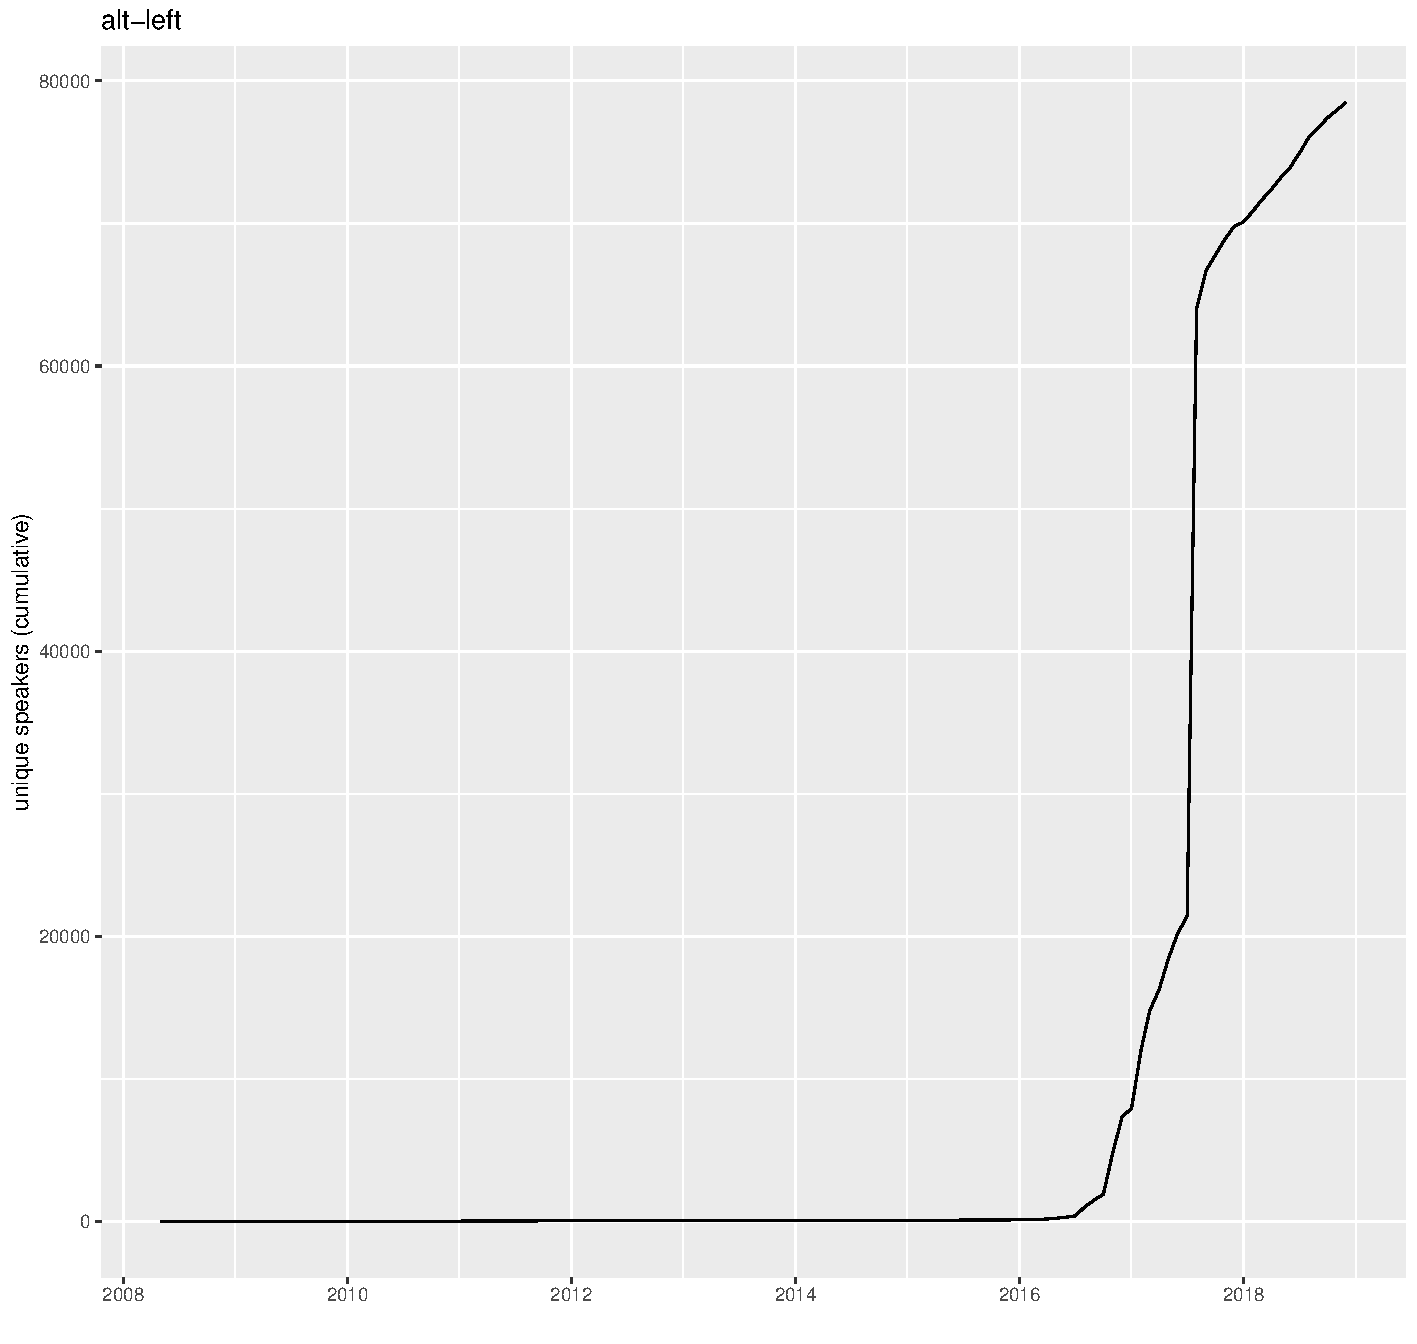
\includegraphics[width=\linewidth, height=.8\textheight, keepaspectratio]{/Users/quirin/promo/sna/out/users/uu_alt-left.pdf}
      \end{subfigure}
      \begin{subfigure}{.45\linewidth}
        \caption{\ol{solopreneur}}
        \centering
        \includegraphics[width=\linewidth, height=.8\textheight, keepaspectratio]{/Users/quirin/promo/sna/out/users/uu_solopreneur.pdf}
      \end{subfigure}
    \end{figure}

  \subsection{Temporal dynamics: coefficient of variation}

    \begin{easylist}[itemize]
      # most volatile candidates: \ol{poppygate}, \ol{burkini} etc.
      # will be excluded from in-depth analyses
    \end{easylist}

  \subsection{Speaker counts}

      I will go beyond frequency and look into the sociolinguistic dynamics more closely

      \begin{easylist}[itemize]
        # sociolinguistic dynamics of diffusion over time
        # sociolinguistic conventionality status of neologism
      \end{easylist}

\section{Diffusion over time}

  \subsection{Advanced: \ol{ghosting}}

    \begin{figure}[H]
      \caption{Usage frequency for \ol{ghosting}.}
      \centering
      \includegraphics[width=\linewidth, height=.8\textheight, keepaspectratio]{/Users/quirin/promo/sna/out/uses/ui_ghosting_time.pdf}
    \end{figure}

    \begin{figure}[H]
      \caption{Social network of diffusion for \ol{ghosting} over time.}
      \centering
      \begin{subfigure}{.45\linewidth}
        \caption{First stage}
        \centering
        \includegraphics[width=\linewidth, height=\textheight, keepaspectratio]{/Users/quirin/promo/sna/gephi/plots/ghosting_one.pdf}
      \end{subfigure}
      \begin{subfigure}{.45\linewidth}
        \caption{Second stage}
        \centering
        \includegraphics[width=\linewidth, height=\textheight, keepaspectratio]{/Users/quirin/promo/sna/gephi/plots/ghosting_two.pdf}
      \end{subfigure}\\
      \begin{subfigure}{.45\linewidth}
        \caption{Third stage}
        \centering
        \includegraphics[width=\linewidth, height=\textheight, keepaspectratio]{/Users/quirin/promo/sna/gephi/plots/ghosting_three.pdf}
      \end{subfigure}
      \begin{subfigure}{.45\linewidth}
        \caption{Fourth stage}
        \centering
        \includegraphics[width=\linewidth, height=\textheight, keepaspectratio]{/Users/quirin/promo/sna/gephi/plots/ghosting_four.pdf}
      \end{subfigure}
    \end{figure}

  \subsection{Advanced: \ol{upcycling}}

    \begin{figure}[H]
      \caption{Usage frequency for \ol{upcycling}.}
      \centering
      \includegraphics[width=\linewidth, height=.8\textheight, keepaspectratio]{/Users/quirin/promo/sna/out/uses/ui_upcycling_time.pdf}
    \end{figure}

    \begin{figure}[H]
      \caption{Social network of diffusion for \ol{upcycling} over time.}
      \centering
      \begin{subfigure}{.45\linewidth}
        \caption{First stage}
        \centering
        \includegraphics[width=\linewidth, height=\textheight, keepaspectratio]{/Users/quirin/promo/sna/gephi/plots/upcycling_one.pdf}
      \end{subfigure}
      \begin{subfigure}{.45\linewidth}
        \caption{Second stage}
        \centering
        \includegraphics[width=\linewidth, height=\textheight, keepaspectratio]{/Users/quirin/promo/sna/gephi/plots/upcycling_two.pdf}
      \end{subfigure}\\
      \begin{subfigure}{.45\linewidth}
        \caption{Third stage}
        \centering
        \includegraphics[width=\linewidth, height=\textheight, keepaspectratio]{/Users/quirin/promo/sna/gephi/plots/upcycling_three.pdf}
      \end{subfigure}
      \begin{subfigure}{.45\linewidth}
        \caption{Fourth stage}
        \centering
        \includegraphics[width=\linewidth, height=\textheight, keepaspectratio]{/Users/quirin/promo/sna/gephi/plots/upcycling_four.pdf}
      \end{subfigure}
    \end{figure}

  \subsection{Increasing diffusion: \ol{lituation}}

    \begin{figure}[H]
      \caption{Usage frequency of \ol{lituation} over time.}
      \centering
      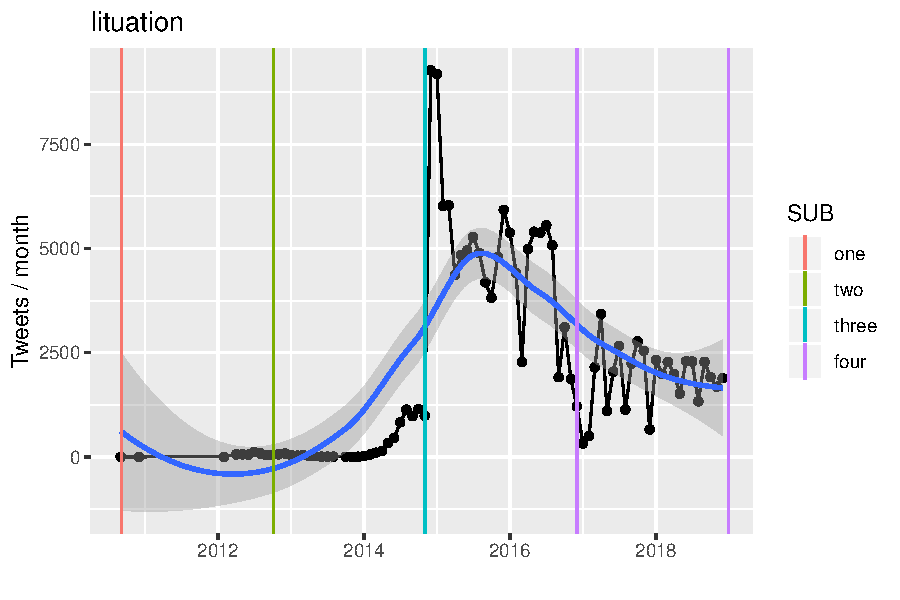
\includegraphics[width=\linewidth, height=.8\textheight, keepaspectratio]{/Users/quirin/promo/sna/out/uses/ui_lituation_time.pdf}
    \end{figure}

    \begin{figure}[H]
      \caption{Social network of diffusion for \ol{lituation} over time.}
      \centering
      \begin{subfigure}{.45\linewidth}
        \caption{First stage}
        \centering
        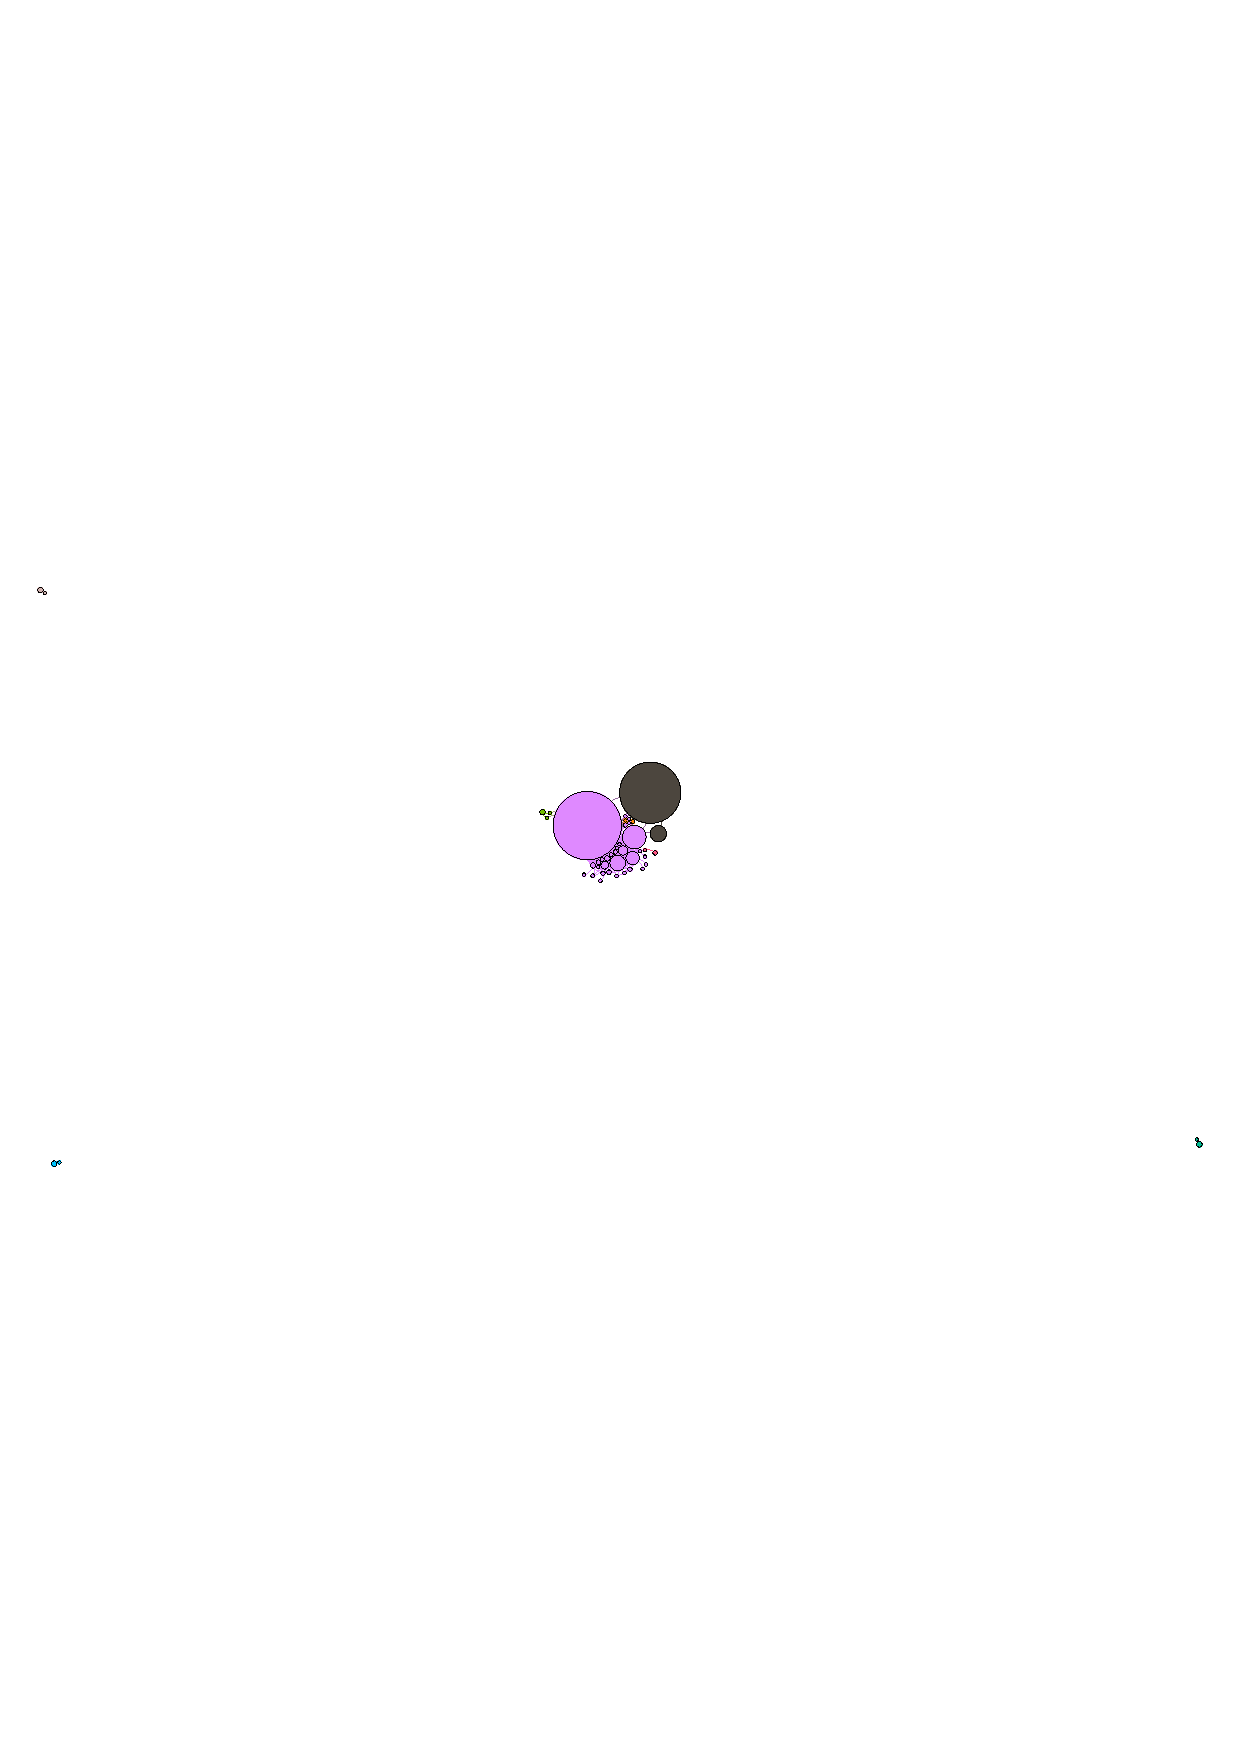
\includegraphics[width=\linewidth, height=\textheight, keepaspectratio]{/Users/quirin/promo/sna/gephi/plots/lituation_one.pdf}
      \end{subfigure}
      \begin{subfigure}{.45\linewidth}
        \caption{Second stage}
        \centering
        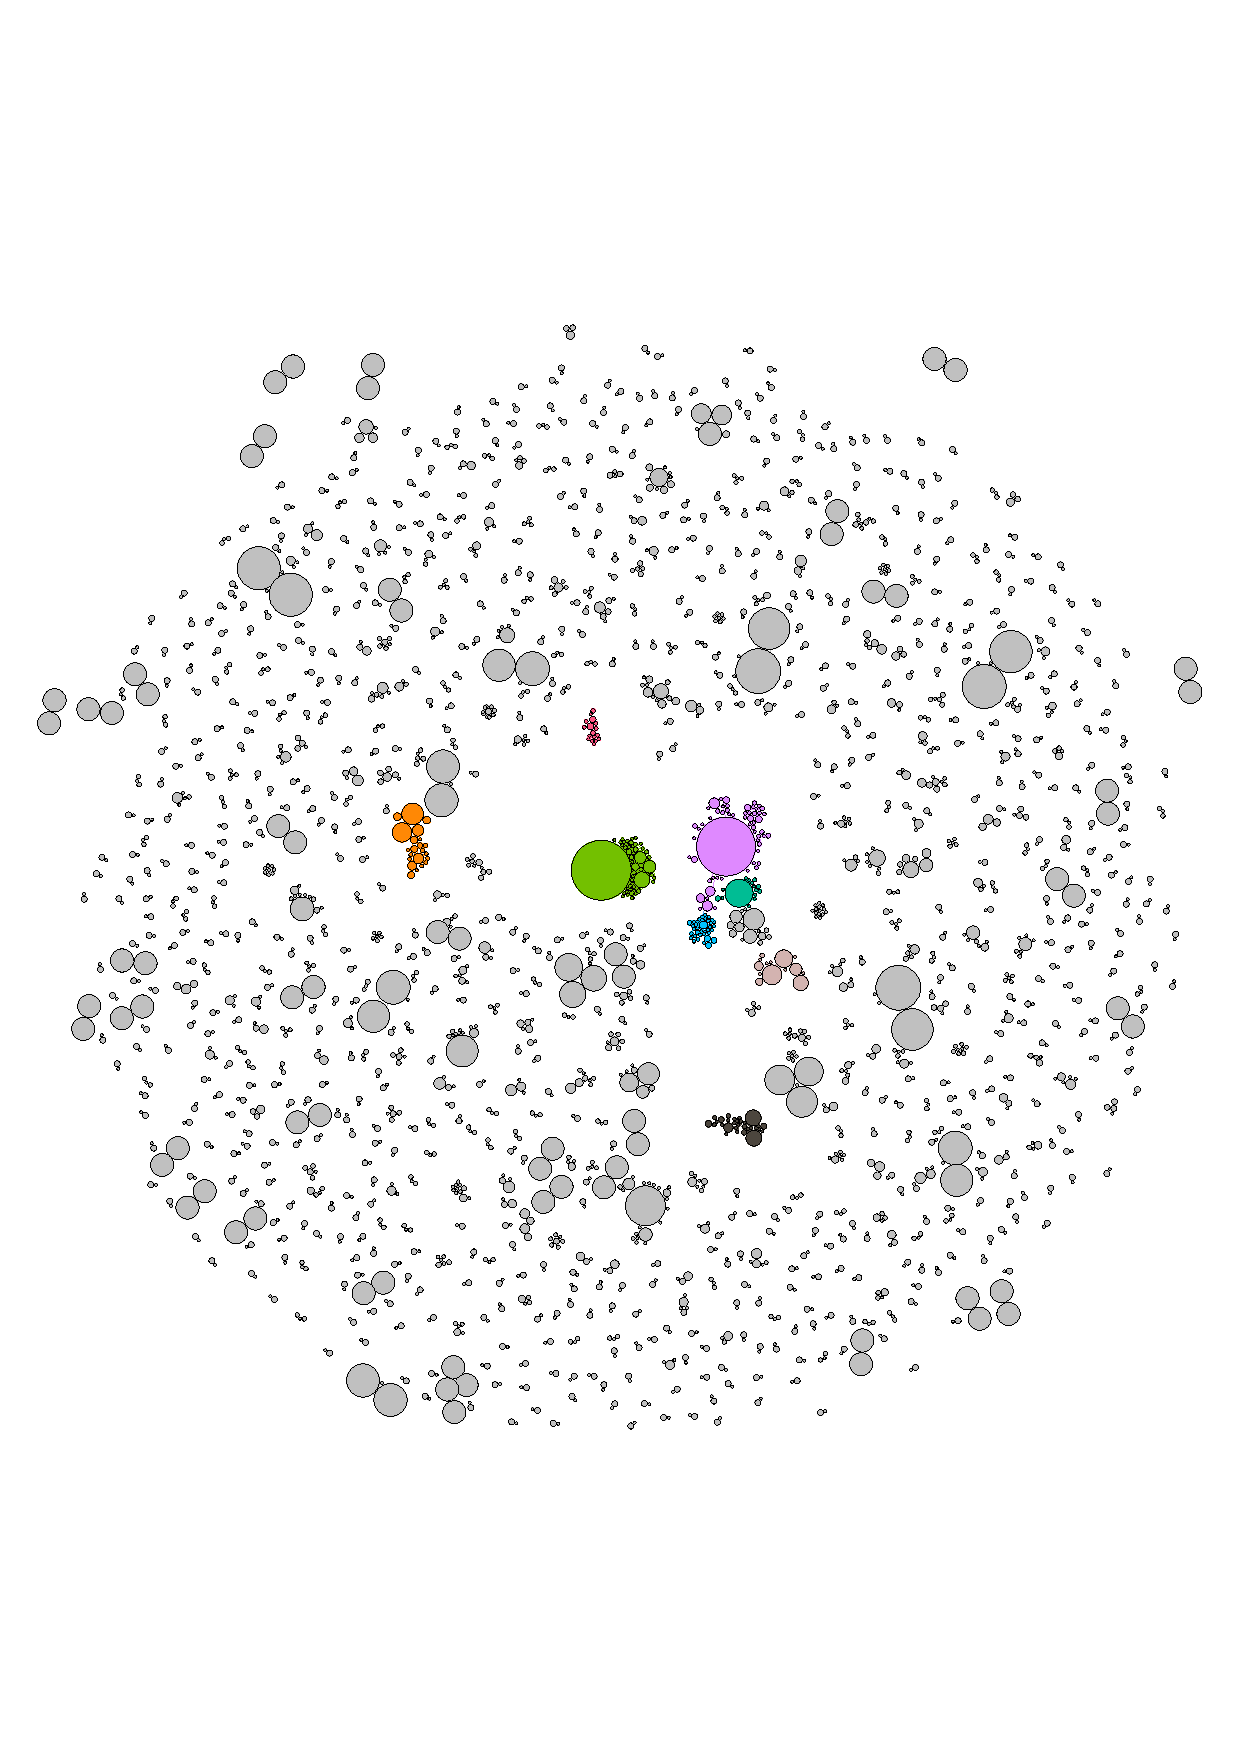
\includegraphics[width=\linewidth, height=\textheight, keepaspectratio]{/Users/quirin/promo/sna/gephi/plots/lituation_two.pdf}
      \end{subfigure}\\
      \begin{subfigure}{.45\linewidth}
        \caption{Third stage}
        \centering
        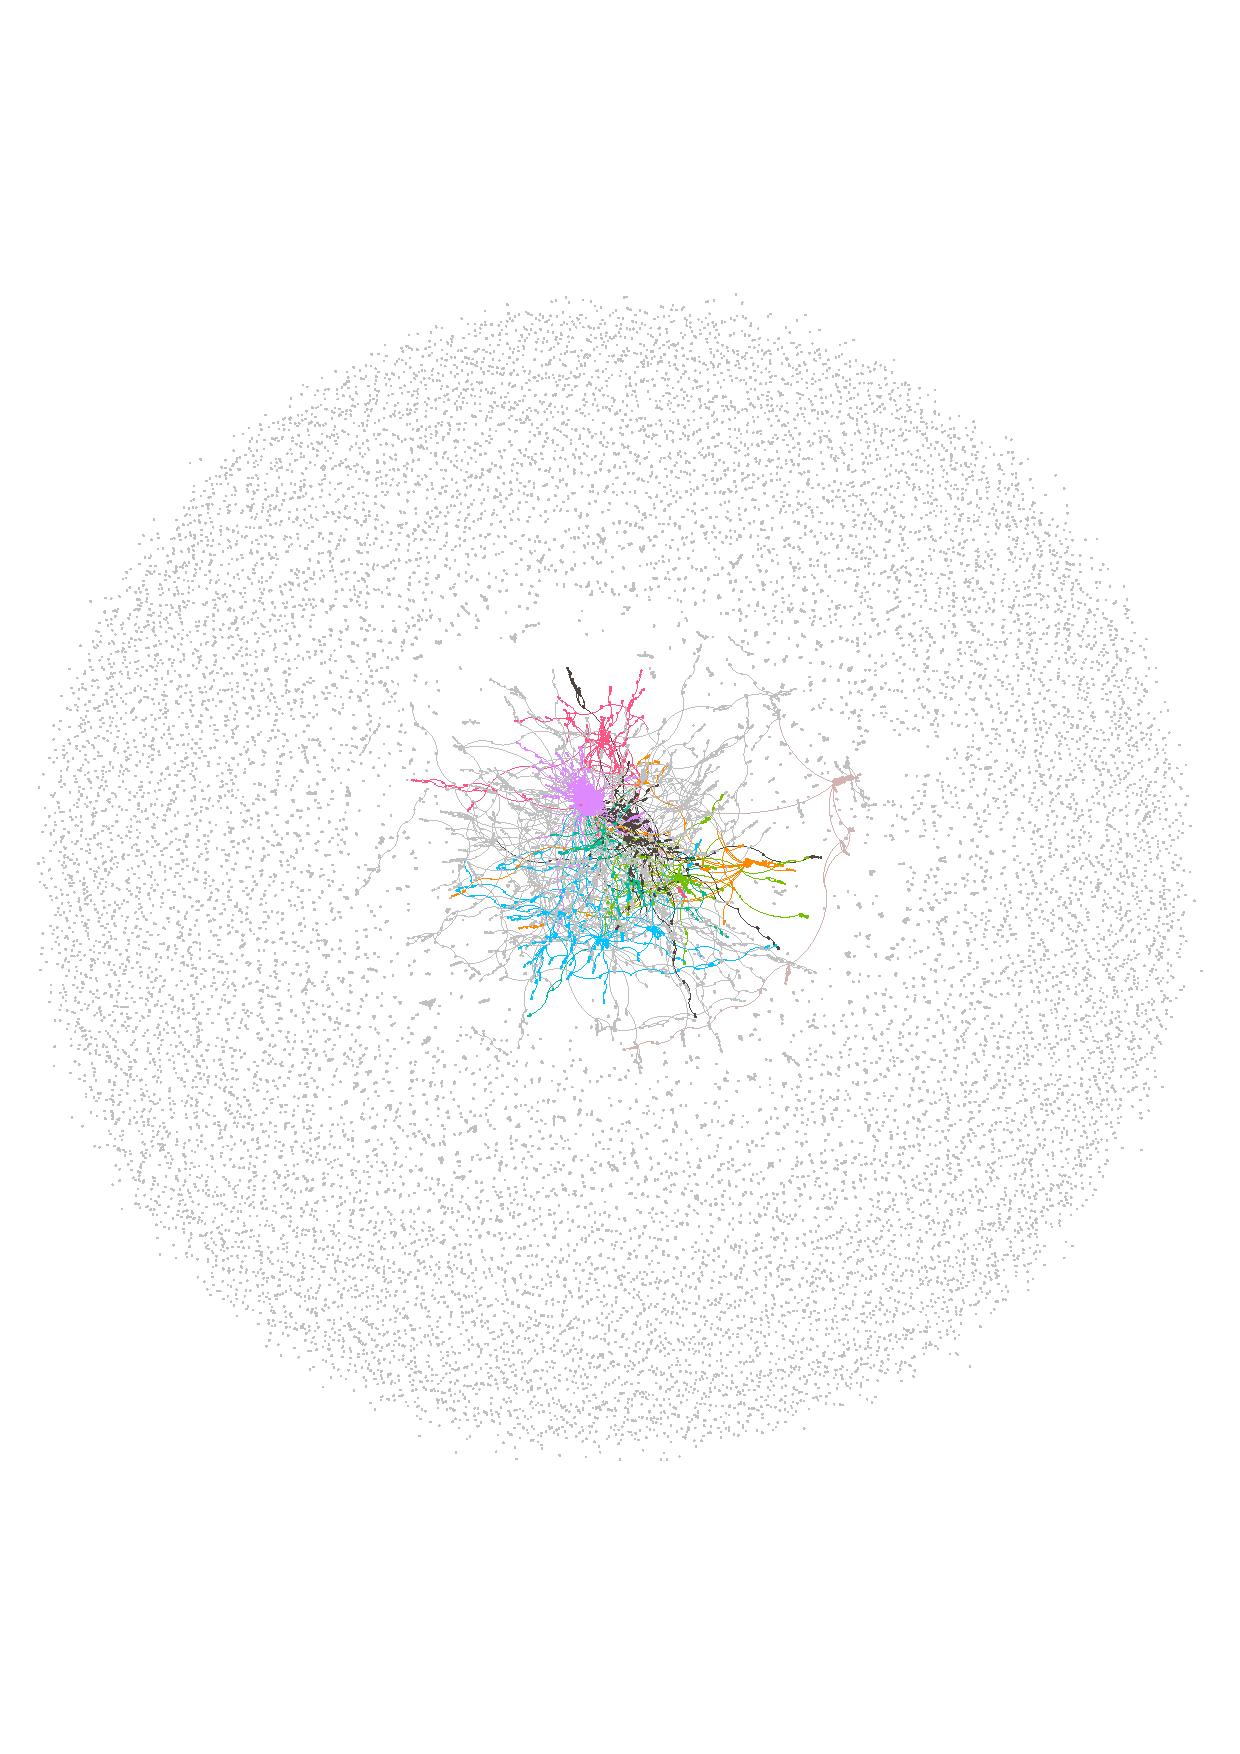
\includegraphics[width=\linewidth, height=\textheight, keepaspectratio]{/Users/quirin/promo/sna/gephi/plots/lituation_three.pdf}
      \end{subfigure}
      \begin{subfigure}{.45\linewidth}
        \caption{Fourth stage}
        \centering
        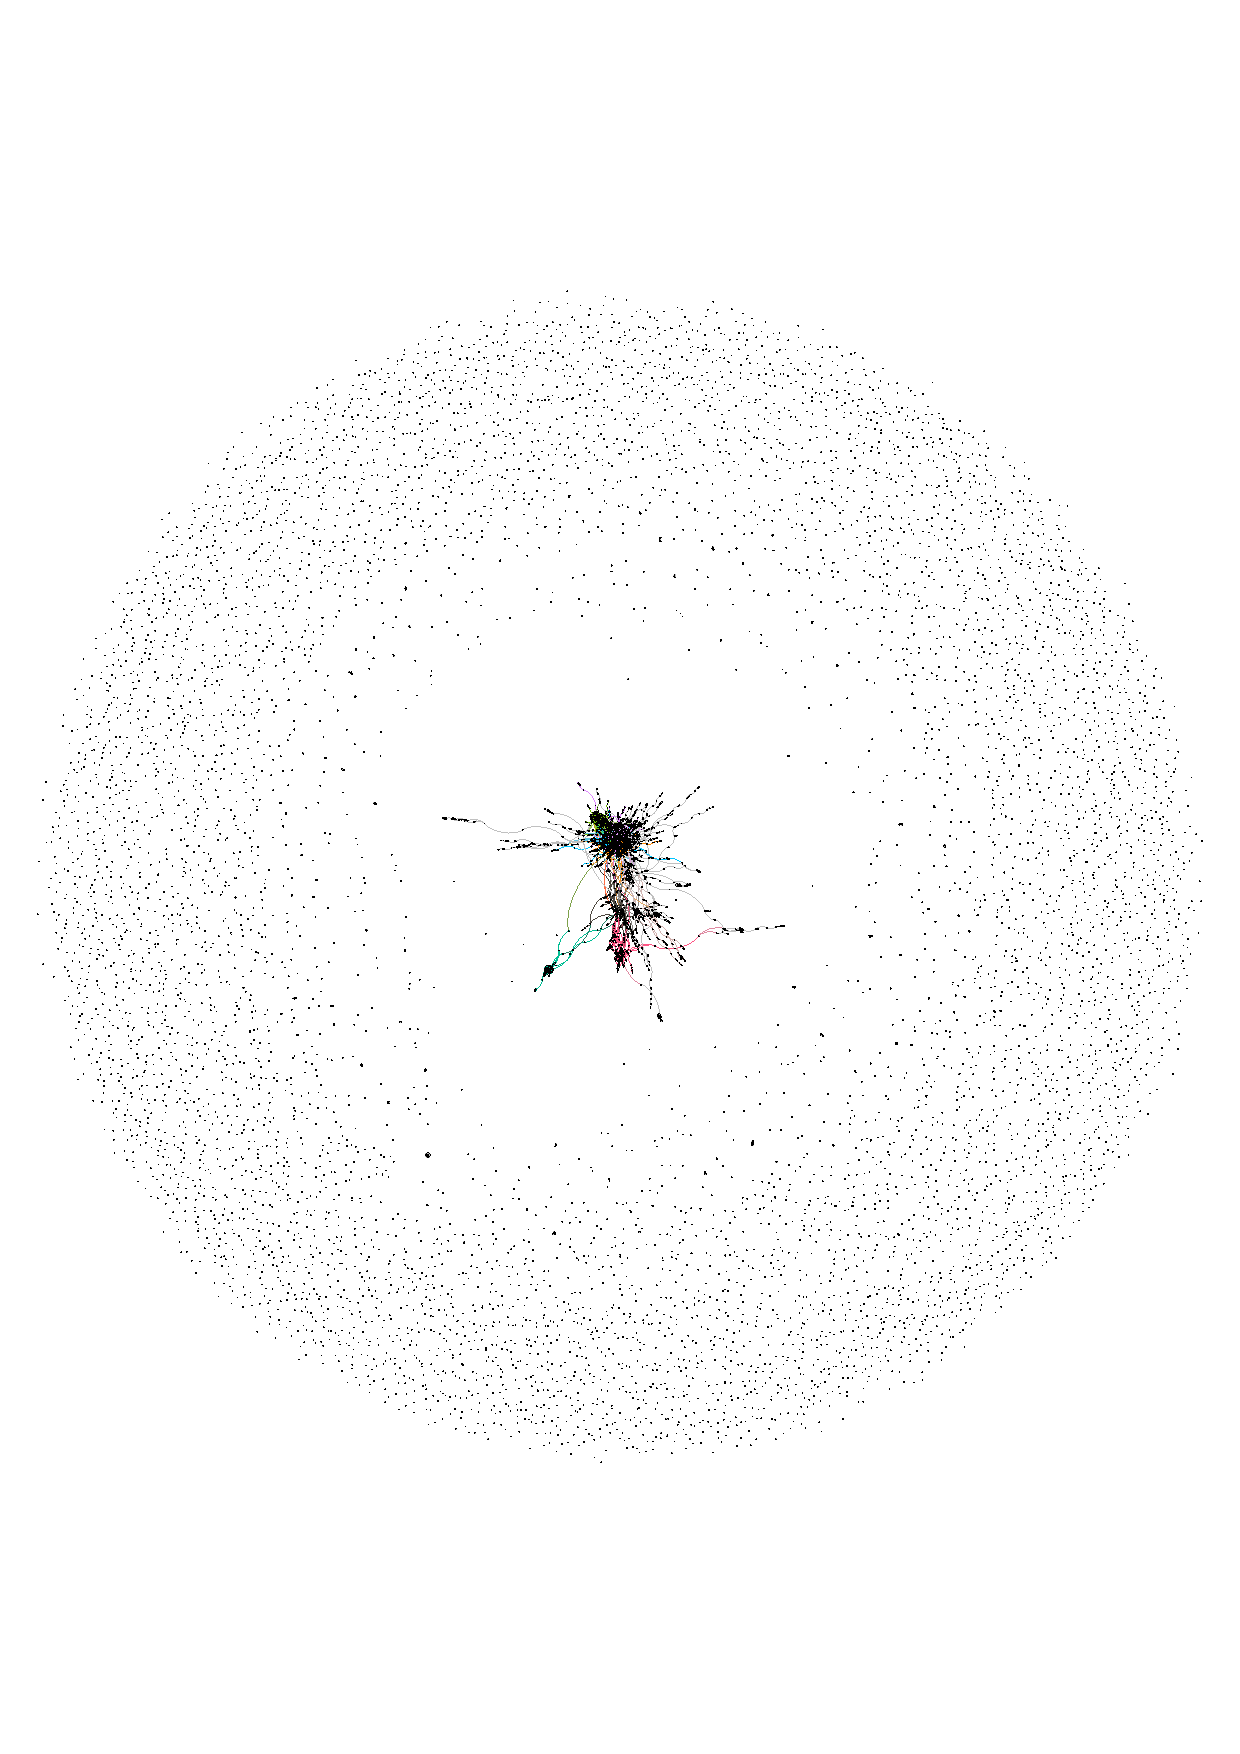
\includegraphics[width=\linewidth, height=\textheight, keepaspectratio]{/Users/quirin/promo/sna/gephi/plots/lituation_four.pdf}
      \end{subfigure}
    \end{figure}

  \subsection{Centralized use: \ol{alt-left}}

    \begin{figure}[H]
      \caption{Usage frequency of \ol{alt-left} over time.}
      \centering
      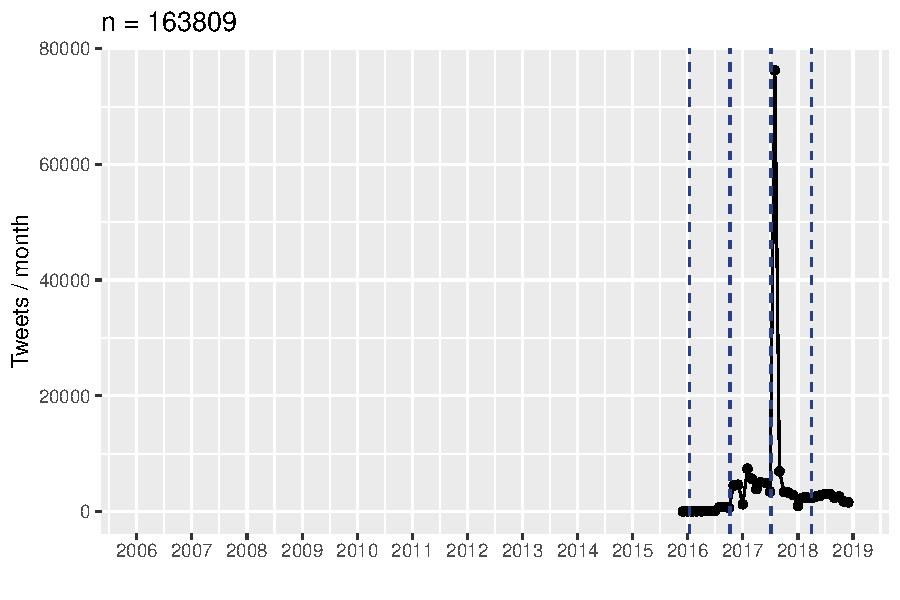
\includegraphics[width=\linewidth, height=.8\textheight, keepaspectratio]{/Users/quirin/promo/sna/out/uses/ui_alt-left_time.pdf}
    \end{figure}

    \begin{figure}[H]
      \caption{Social network of diffusion for \ol{alt-left} over time.}
      \centering
      \begin{subfigure}{.45\linewidth}
        \caption{First stage}
        \centering
        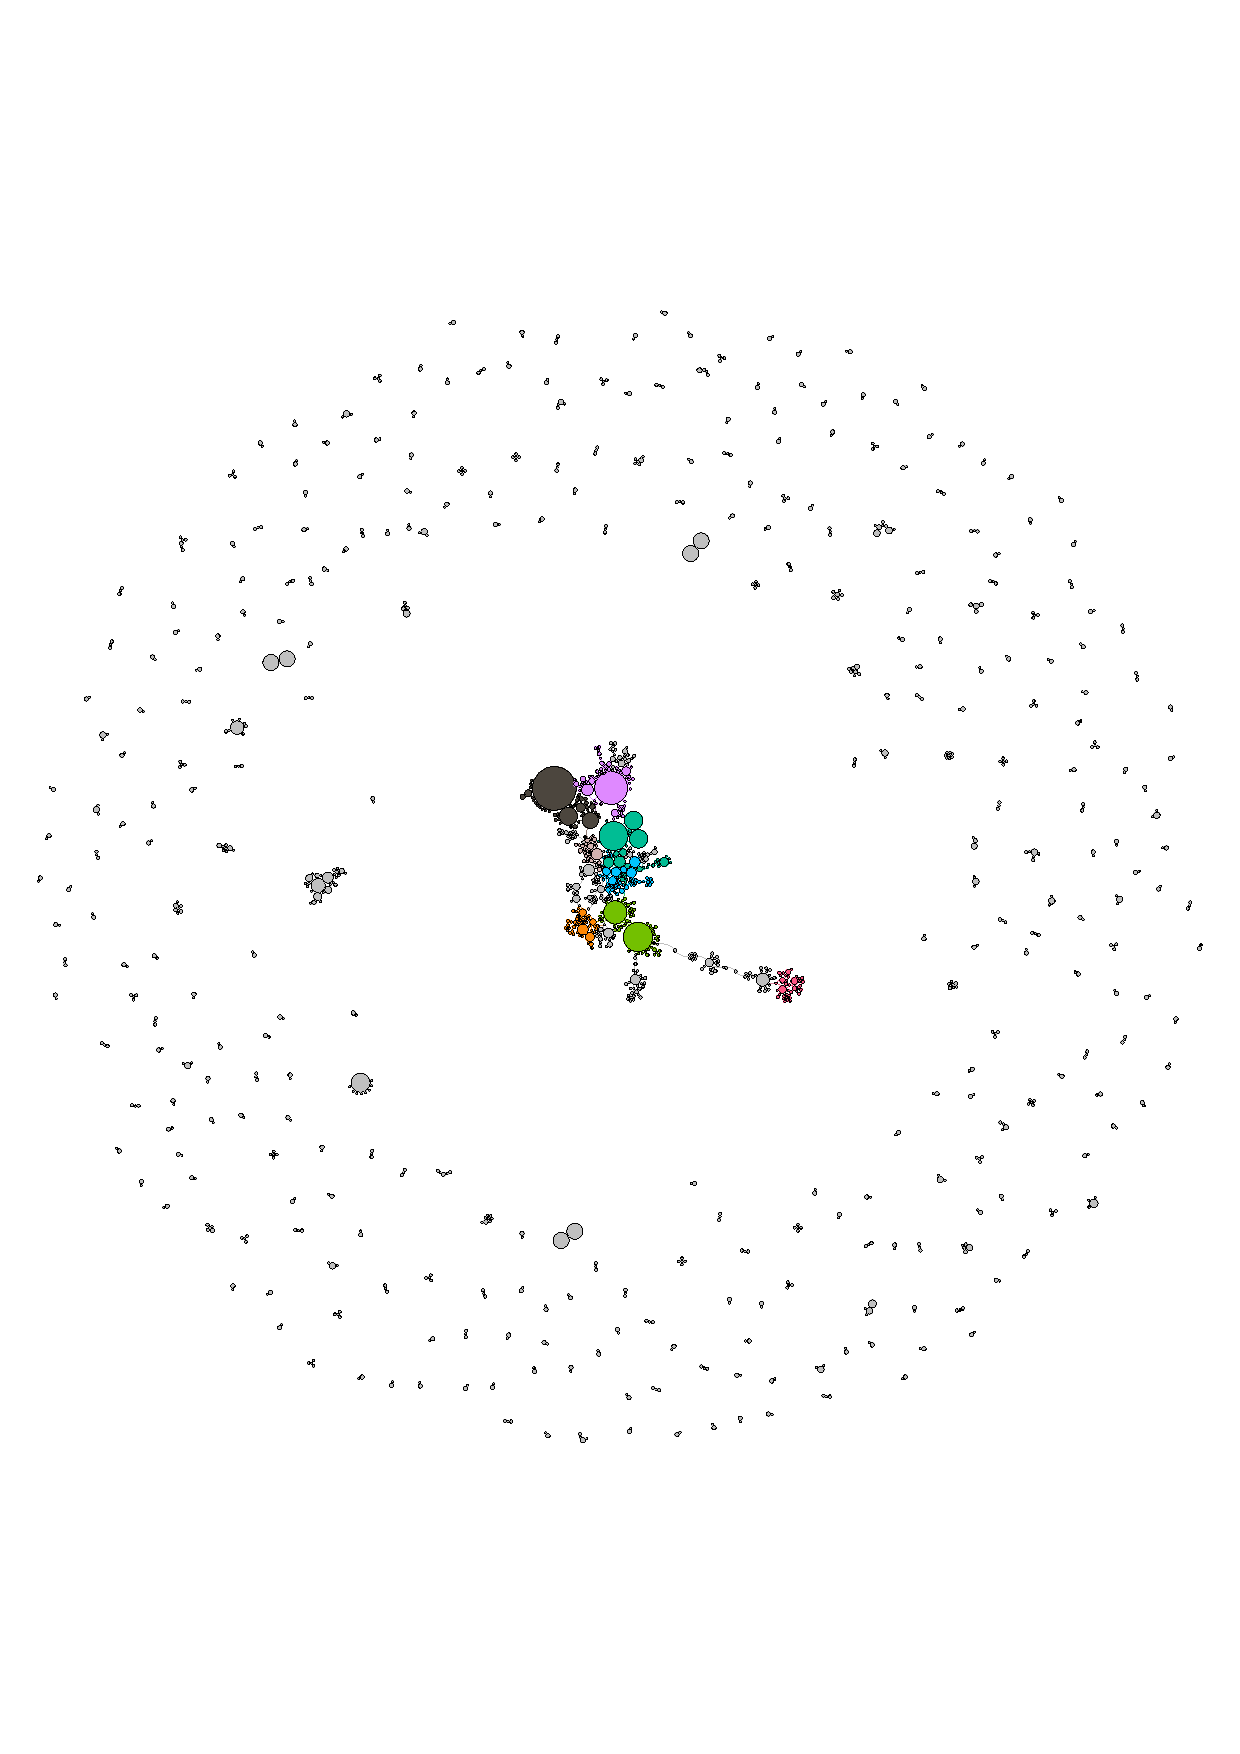
\includegraphics[width=\linewidth, height=\textheight, keepaspectratio]{/Users/quirin/promo/sna/gephi/plots/alt-left_one.pdf}
      \end{subfigure}
      \begin{subfigure}{.45\linewidth}
        \caption{Second stage}
        \centering
        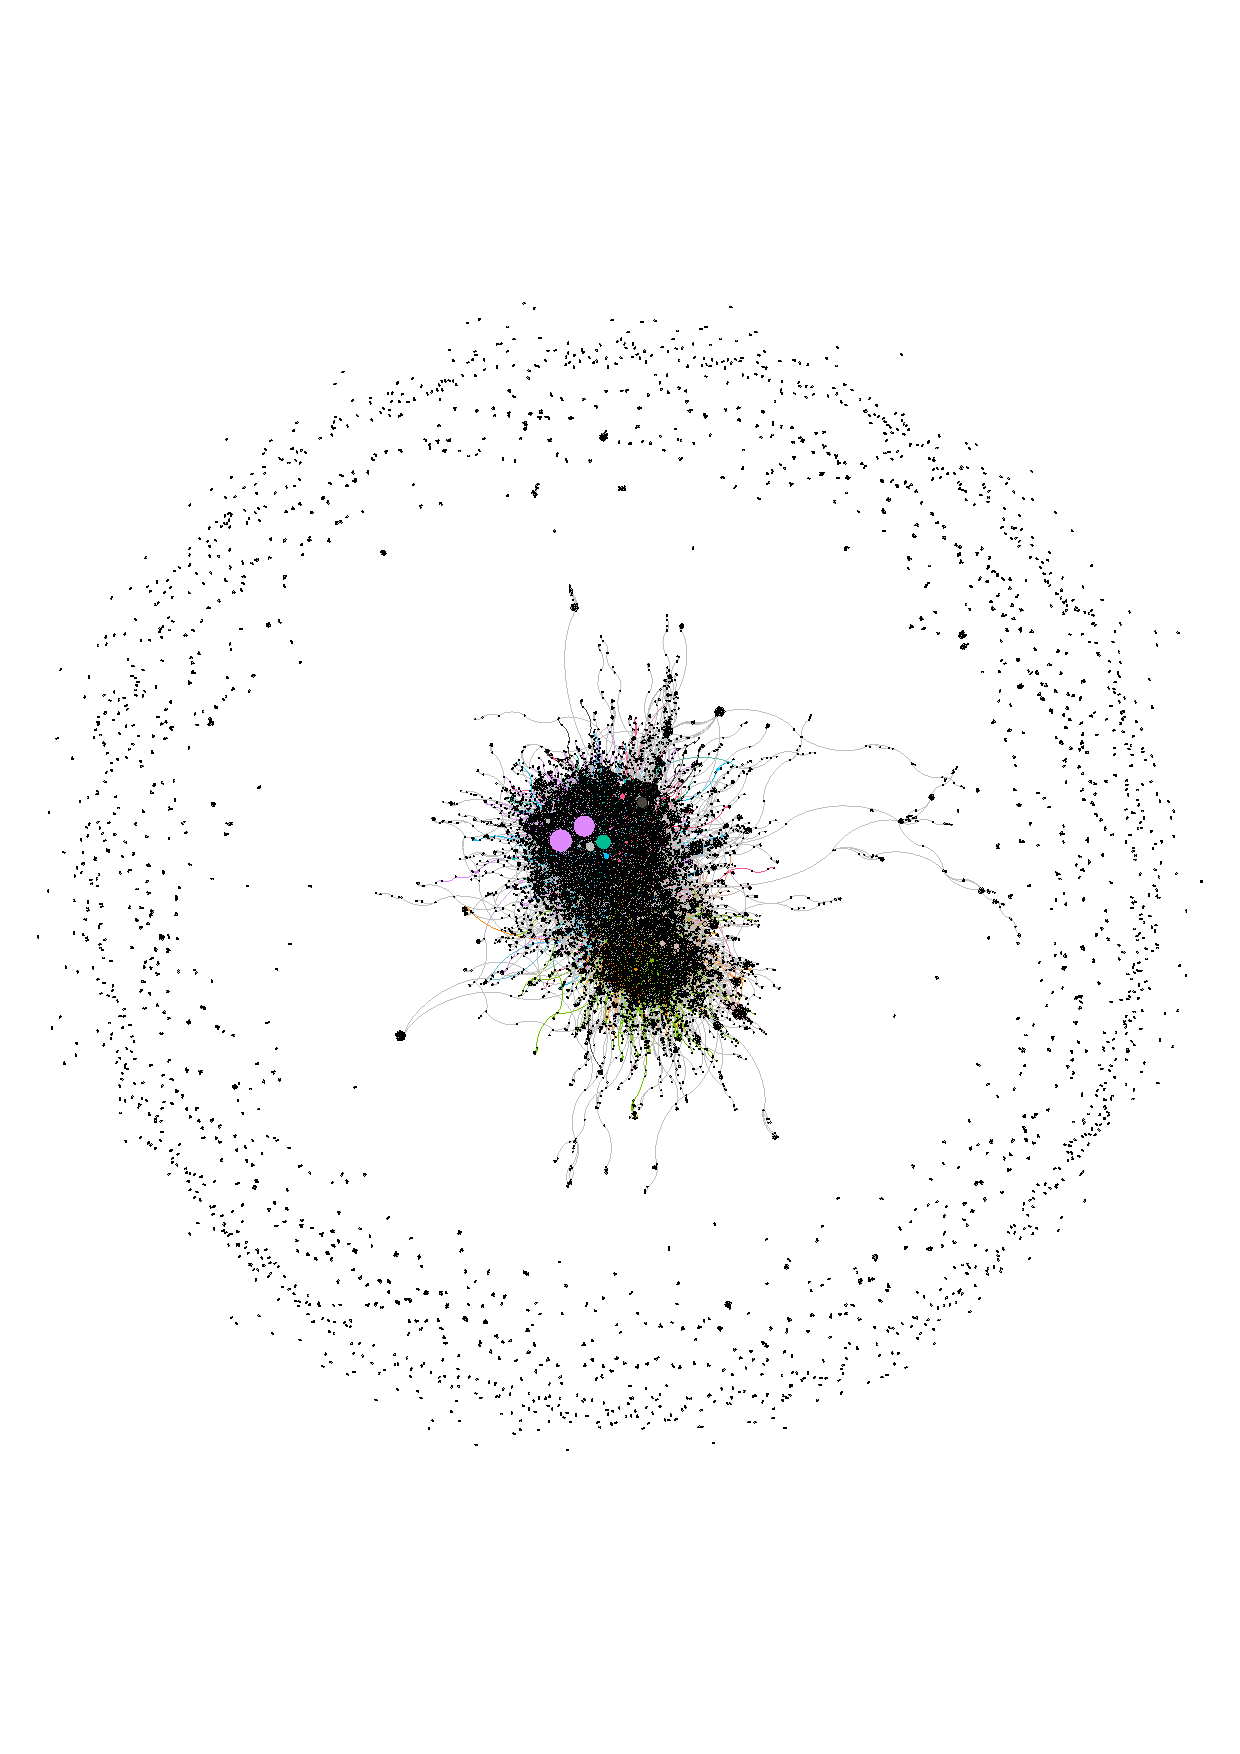
\includegraphics[width=\linewidth, height=\textheight, keepaspectratio]{/Users/quirin/promo/sna/gephi/plots/alt-left_two.pdf}
      \end{subfigure}\\
      \begin{subfigure}{.45\linewidth}
        \caption{Third stage}
        \centering
        \includegraphics[width=\linewidth, height=\textheight, keepaspectratio]{/Users/quirin/promo/sna/gephi/plots/alt-left_three.pdf}
      \end{subfigure}
      \begin{subfigure}{.45\linewidth}
        \caption{Fourth stage}
        \centering
        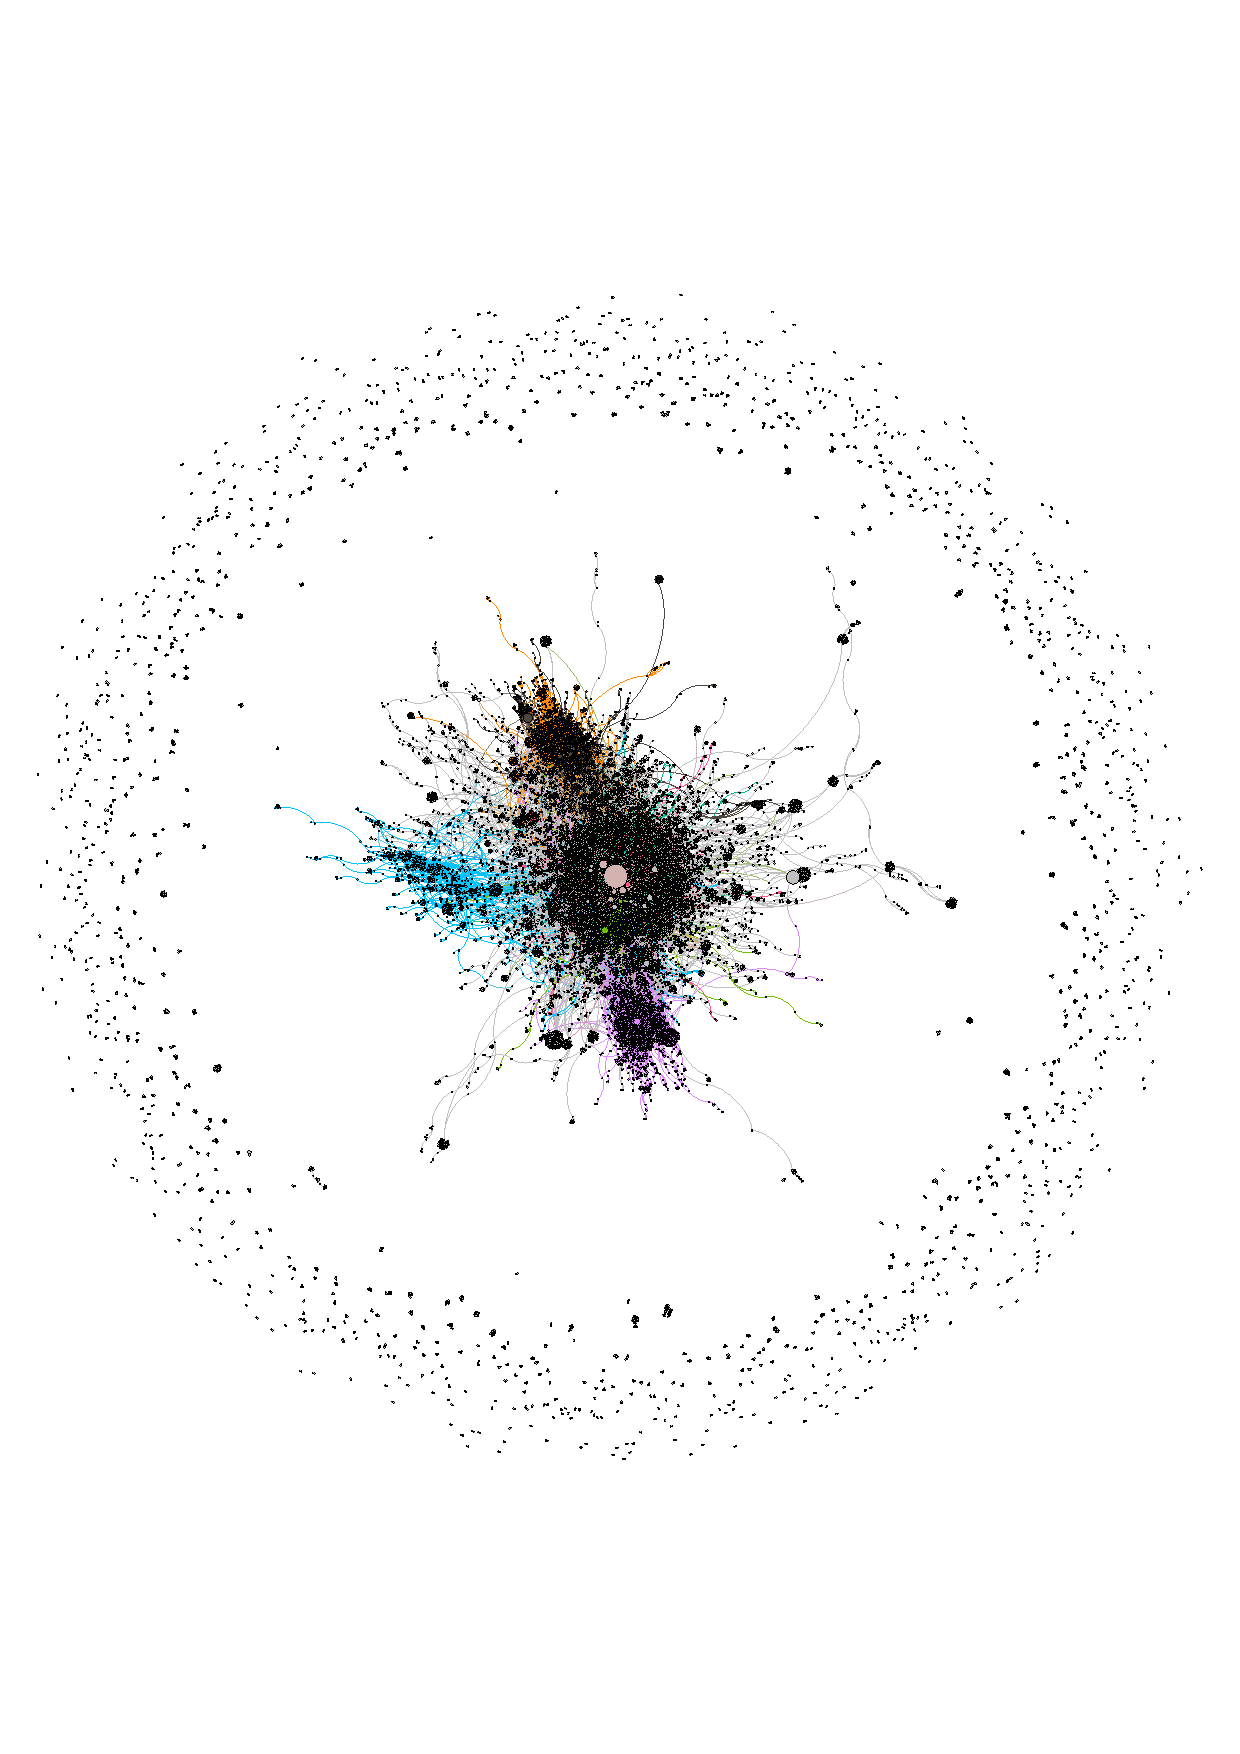
\includegraphics[width=\linewidth, height=\textheight, keepaspectratio]{/Users/quirin/promo/sna/gephi/plots/alt-left_four.pdf}
      \end{subfigure}
    \end{figure}

  \subsection{Narrowing: \ol{solopreneur}}

    \begin{figure}[H]
      \caption{Usage frequency of \ol{solopreneur} over time.}
      \centering
      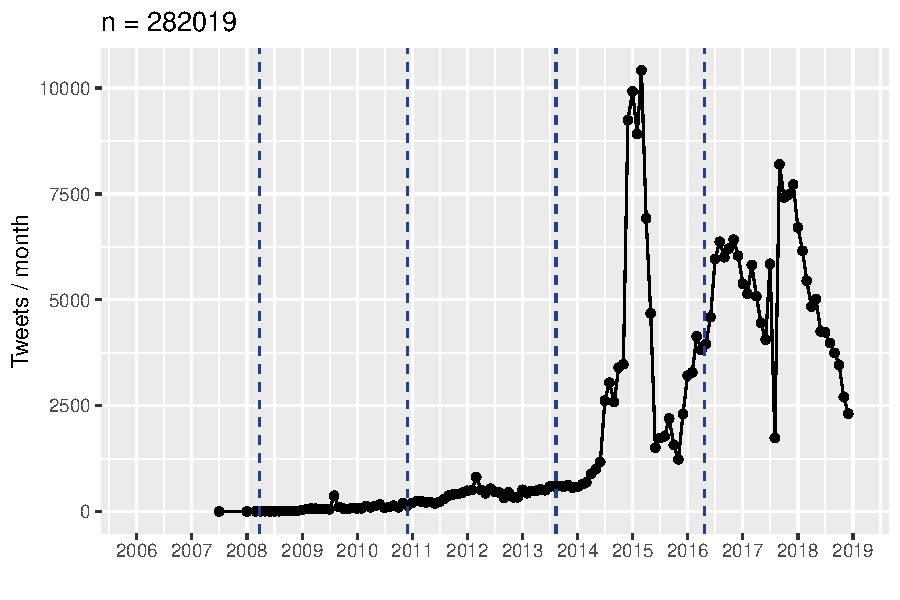
\includegraphics[width=\linewidth, height=.8\textheight, keepaspectratio]{/Users/quirin/promo/sna/out/uses/ui_solopreneur_time.pdf}
    \end{figure}

    \begin{figure}[H]
      \caption{Social network of diffusion for \ol{solopreneur} over time.}
      \centering
      % \begin{subfigure}{.45\linewidth}
      %   \caption{First stage}
      %   \centering
      %   \includegraphics[width=\linewidth, height=\textheight, keepaspectratio]{/Users/quirin/promo/sna/gephi/plots/solopreneur_one.pdf}
      % \end{subfigure}
      % \begin{subfigure}{.45\linewidth}
      %   \caption{Second stage}
      %   \centering
      %   \includegraphics[width=\linewidth, height=\textheight, keepaspectratio]{/Users/quirin/promo/sna/gephi/plots/solopreneur_two.pdf}
      % \end{subfigure}\\
      % \begin{subfigure}{.45\linewidth}
      %   \caption{Third stage}
      %   \centering
      %   \includegraphics[width=\linewidth, height=\textheight, keepaspectratio]{/Users/quirin/promo/sna/gephi/plots/solopreneur_three.pdf}
      % \end{subfigure}
      % \begin{subfigure}{.45\linewidth}
      %   \caption{Fourth stage}
      %   \centering
      %   \includegraphics[width=\linewidth, height=\textheight, keepaspectratio]{/Users/quirin/promo/sna/gephi/plots/solopreneur_four.pdf}
      % \end{subfigure}
    \end{figure}

  \subsection{Overall diachronic development for case studies}

    \begin{figure}[H]
      \caption{Degree centralization over time for case study words.}
      \centering
      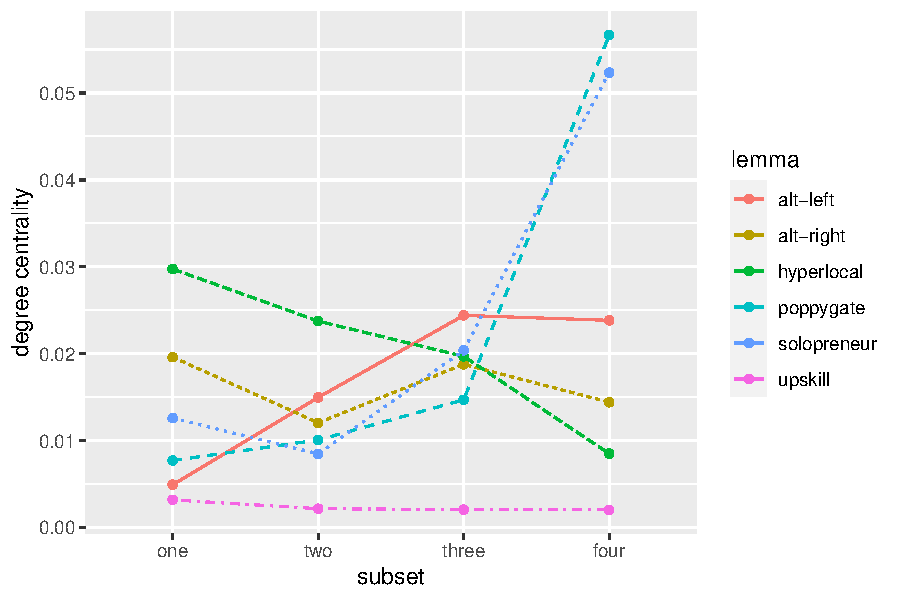
\includegraphics[width=\linewidth, height=.8\textheight, keepaspectratio]{/Users/quirin/promo/sna/out/cases_cent_diac.pdf}
    \end{figure}

\section{Full sample}

  \subsection{Diachronic development}

    \begin{figure}
      \caption{Degree centralization over time for the full sample.}
      \centering
      \includegraphics[width=\linewidth, height=.8\textheight, keepaspectratio]{/Users/quirin/promo/sna/out/full_cent_diac.pdf}
    \end{figure}

  \subsection{Biggest changes}

    \begin{easylist}[itemize]
      # increasing diffusion
      # centralization
    \end{easylist}

\section{Networks vs. frequency}

  \subsection{Plots}

    \begin{figure}
      \centering
      \begin{subfigure}{.45\linewidth}
        \caption{Full sample.}
        \centering
        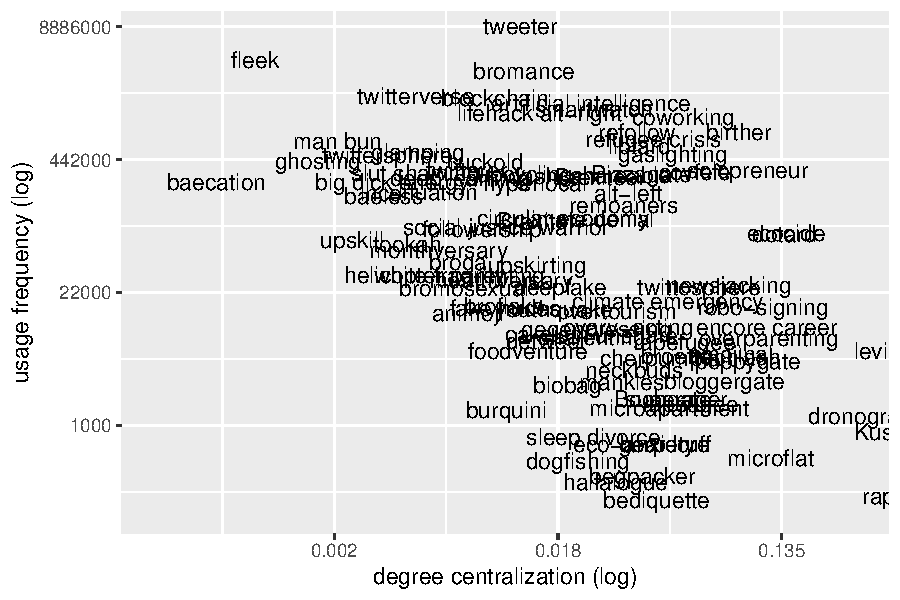
\includegraphics[width=\linewidth, height=.8\textheight, keepaspectratio]{/Users/quirin/promo/sna/out/full_cent_freq_overall.pdf}
      \end{subfigure}
      \begin{subfigure}{.45\linewidth}
        \caption{Case studies.}
        \centering
        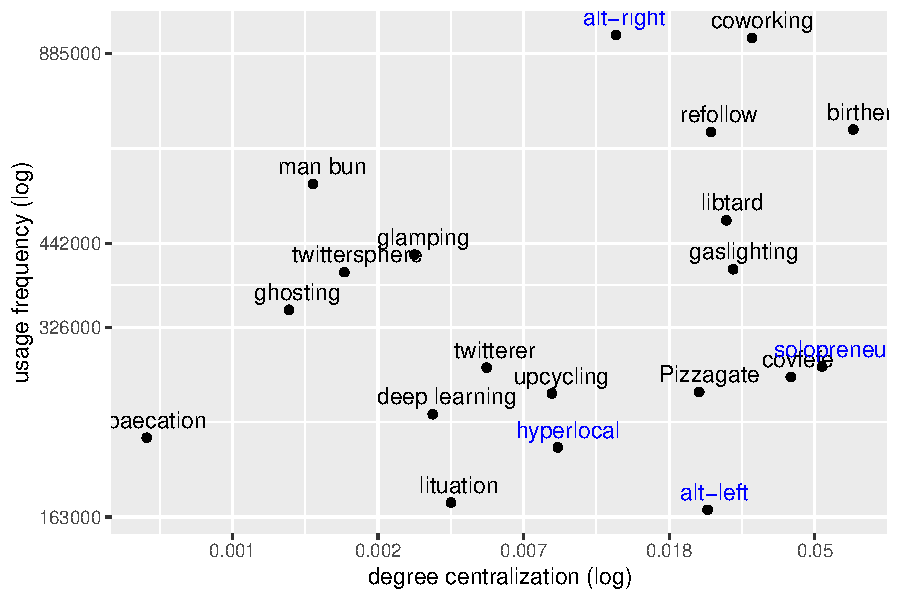
\includegraphics[width=\linewidth, height=.8\textheight, keepaspectratio]{/Users/quirin/promo/sna/out/cases_cent_freq_overall.pdf}
      \end{subfigure}
    \end{figure}

  \subsection{Correlation}

  \subsection{Grouping and interpretation}

    Divergences between frequency and network analysis

      \begin{easylist}[itemize]
        # advanced
        # topical
        # little dispersion
          ## political camps:
            ### propaganda: \ol{alt-right}, \ol{alt-left}, \ol{covfefe}, \ol{birther}
            ### Brexit terms: \ol{Brexiteer}, \ol{Brexiter}, \ol{Brexit}
          ## technical
      \end{easylist}

    $\rightarrow$ case studies

\section{Conclusion}

  \begin{easylist}[itemize]
    # going beyond frequency is important
  \end{easylist}

% bibliography

  \printbibliography

\end{document}
